\documentclass[a4paper, 11pt]{article}
\usepackage[python,linenum]{mypackage}
\usepackage{amsmath}
\usepackage{graphicx}
\usepackage{geometry}
\geometry{scale=0.8}
\usepackage{hyperref}
\usepackage{enumitem}
\usepackage{color}
\usepackage[linesnumbered,boxed]{algorithm2e}

\setenumerate[1]{itemsep=0pt,partopsep=0pt,parsep=\parskip,topsep=0pt}
\setitemize[1]{itemsep=0pt,partopsep=0pt,parsep=\parskip,topsep=0pt}
\setdescription{itemsep=0pt,partopsep=0pt,parsep=\parskip,topsep=0pt}


\title{
\normalfont \normalsize
\textsc{School of Data and Computer Science, Sun Yat-sen University} \\ [25pt] %textsc small capital letters
\rule{\textwidth}{0.5pt} \\[0.4cm] % Thin top horizontal rule
\huge  E16 Deep Learning (C++/Python)\\ % The assignment title
\rule{\textwidth}{2pt} \\[0.5cm] % Thick bottom horizontal rule
\author{17341015 Hongzheng Chen}
\date{\normalsize\today}
}

\begin{document}
\maketitle
\tableofcontents
\newpage
\section{The CIFAR-10 dataset}
The CIFAR-10 dataset (\url{http://www.cs.toronto.edu/~kriz/cifar.html}) consists of 60000 $32\times 32$ colour images in 10 classes, with 6000 images per class. There are 50000 training images and 10000 test images.

The dataset is divided into five training batches and one test batch, each with 10000 images. The test batch contains exactly 1000 randomly-selected images from each class. The training batches contain the remaining images in random order, but some training batches may contain more images from one class than another. Between them, the training batches contain exactly 5000 images from each class. Here are the classes in the dataset, as well as 10 random images from each:
\begin{figure}[H]
\centering
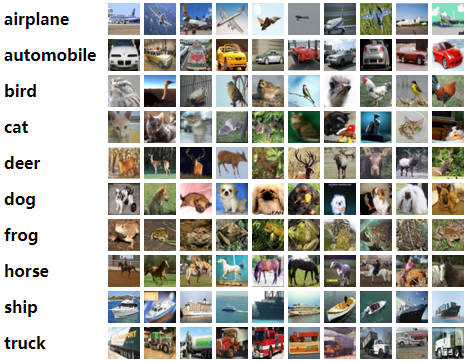
\includegraphics[width=0.5\textwidth]{fig/cifar}
\end{figure}

The classes are completely mutually exclusive. There is no overlap between automobiles and trucks. "Automobile" includes sedans, SUVs, things of that sort. "Truck" includes only big trucks. Neither includes pickup trucks.
\section{Convolutional Neural Networks (CNNs / ConvNets)}
Chinese version: \url{https://www.zybuluo.com/hanbingtao/note/485480}\\
English version: \url{http://cs231n.github.io/convolutional-networks/#layers}
\subsection{Architecture Overview}
Regular Neural Nets don’t scale well to full images. In CIFAR-10, images are only of size $32\times 32\times 3$ (32 wide, 32 high, 3 color channels), so a single fully-connected neuron in a first hidden layer of a regular Neural Network would have $32*32*3$ = 3072 weights. This amount still seems manageable, but clearly this fully-connected structure does not scale to larger images. For example, an image of more respectable size, e.g. $200\times 200\times 3$, would lead to neurons that have 200*200*3 = 120,000 weights. Moreover, we would almost certainly want to have several such neurons, so the parameters would add up quickly! Clearly, this full connectivity is wasteful and the huge number of parameters would quickly lead to overfitting.

Convolutional Neural Networks take advantage of the fact that the input consists of images and they constrain the architecture in a more sensible way. In particular, unlike a regular Neural Network, the layers of a ConvNet have neurons arranged in 3 dimensions: width, height, depth. (Note that the word depth here refers to the third dimension of an activation volume, not to the depth of a full Neural Network, which can refer to the total number of layers in a network.) For example, the input images in CIFAR-10 are an input volume of activations, and the volume has dimensions $32\times 32\times 3$ (width, height, depth respectively). As we will soon see, the neurons in a layer will only be connected to a small region of the layer before it, instead of all of the neurons in a fully-connected manner. Moreover, the final output layer would for CIFAR-10 have dimensions $1\times 1\times 10$, because by the end of the ConvNet architecture we will reduce the full image into a single vector of class scores, arranged along the depth dimension. Here is a visualization:
\begin{figure}[H]
\centering
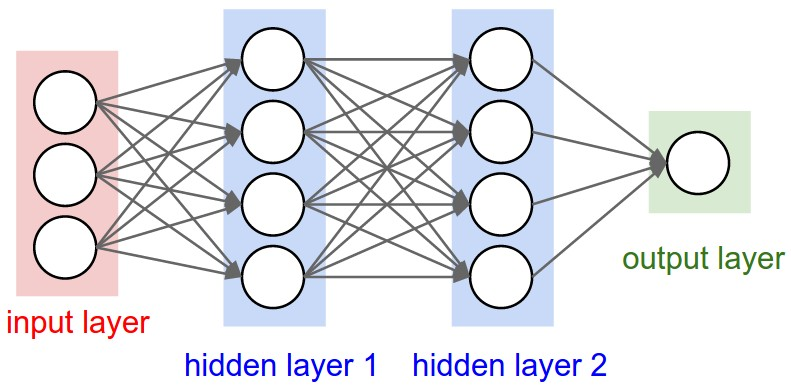
\includegraphics[width=0.4\textwidth]{fig/neural_net2}
\quad
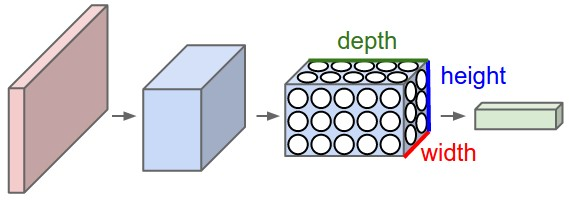
\includegraphics[width=0.4\textwidth]{fig/cnn}
\caption*{Left: A regular 3-layer Neural Network. Right: A ConvNet arranges its neurons in three dimensions (width, height, depth), as visualized in one of the layers. Every layer of a ConvNet transforms the 3D input volume to a 3D output volume of neuron activations. In this example, the red input layer holds the image, so its width and height would be the dimensions of the image, and the depth would be 3 (Red, Green, Blue channels).}
\end{figure}
\begin{figure}
\centering
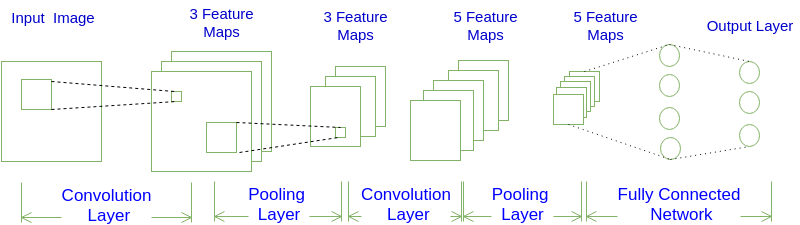
\includegraphics[width=\textwidth]{fig/cnn2}
\end{figure}
\subsection{Layers used to build ConvNets}
a simple ConvNet is a sequence of layers, and every layer of a ConvNet transforms one volume of activations to another through a differentiable function. We use three main types of layers to build ConvNet architectures: \textbf{Convolutional Layer}, \textbf{Pooling Layer}, and \textbf{Fully-Connected Layer} (exactly as seen in regular Neural Networks). We will stack these layers to form a full ConvNet architecture.

\emph{Example Architecture}: Overview. We will go into more details below, but a simple ConvNet for CIFAR-10 classification could have the architecture [\textbf{INPUT - CONV - RELU - POOL - FC}]. In more detail:

\begin{itemize}
	\item INPUT [$32\times 32\times 3$] will hold the raw pixel values of the image, in this case an image of width 32, height 32, and with three color channels R,G,B.
	\item CONV layer will compute the output of neurons that are connected to local regions in the input, each computing a dot product between their weights and a small region they are connected to in the input volume. This may result in volume such as [$32\times 32\times 12$] if we decided to use 12 filters.
	\item RELU layer will apply an elementwise activation function, such as the $max(0,x)$ thresholding at zero. This leaves the size of the volume unchanged ([$32\times 32\times 12$]).
	\item POOL layer will perform a downsampling operation along the spatial dimensions (width, height), resulting in volume such as [$16\times 16\times 12$].
	\item FC (i.e. fully-connected) layer will compute the class scores, resulting in volume of size [$1\times 1\times 10$], where each of the 10 numbers correspond to a class score, such as among the 10 categories of CIFAR-10. As with ordinary Neural Networks and as the name implies, each neuron in this layer will be connected to all the numbers in the previous volume.
\end{itemize}
\subsubsection{Convolutional Layer}
To summarize, the Conv Layer:
\begin{itemize}
	\item Accepts a volume of size $W_1\times H_1\times D_1$
	\item Requires four hyperparameters:
	\begin{itemize}
		\item Number of filters $K$,
		\item their spatial extent $F$,
		\item the stride $S$,
		\item the amount of zero padding $P$.
	\end{itemize}
	\item Produces a volume of size $W_2\times H_2\times D_2$ where:
	\begin{itemize}
		\item $W_2=(W_1-F+2P)/S+1$
		\item $H_2=(H_1-F+2P)/S+1$ (i.e. width and height are computed equally by symmetry)
		\item $D_2=K$
	\end{itemize}
	\item With parameter sharing, it introduces $F\cdot F\cdot D_1$ weights per filter, for a total of $(F\cdot F\cdot D_1)\cdot K$ weights and $K$ biases.
	\item In the output volume, the $d$-th depth slice (of size $W_2\times H_2$) is the result of performing a valid convolution of the $d$-th filter over the input volume with a stride of $S$, and then offset by $d$-th bias.
\end{itemize}

A common setting of the hyperparameters is $F=3$,$S=1$,$P=1$. However, there are common conventions and rules of thumb that motivate these hyperparameters.
\begin{figure}[H]
\centering
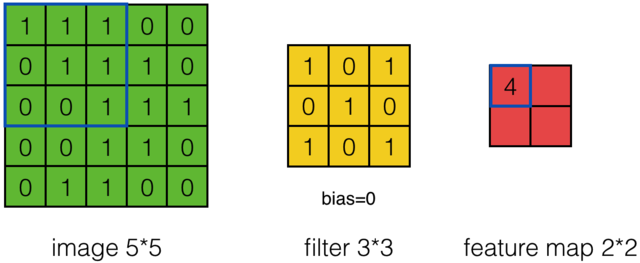
\includegraphics[width=0.8\textwidth]{fig/f1}
\end{figure}
\begin{figure}[H]
\centering
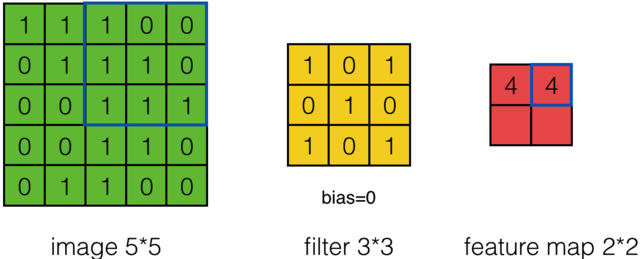
\includegraphics[width=0.8\textwidth]{fig/f2}
\end{figure}
\begin{figure}[H]
\centering
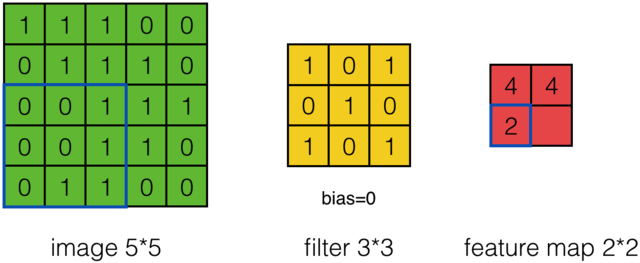
\includegraphics[width=0.8\textwidth]{fig/f3}
\end{figure}
\begin{figure}[H]
\centering
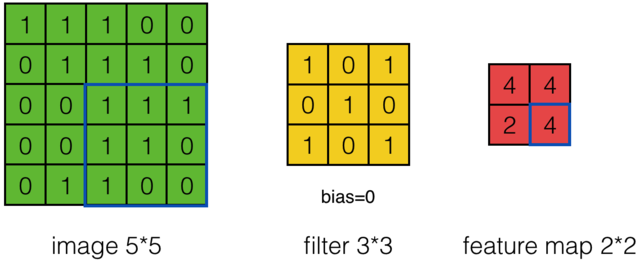
\includegraphics[width=0.8\textwidth]{fig/f4}
\end{figure}
\subsubsection{Pooling Layer}
It is common to periodically insert a Pooling layer in-between successive Conv layers in a ConvNet architecture. Its function is to progressively reduce the spatial size of the representation to reduce the amount of parameters and computation in the network, and hence to also control overfitting. The Pooling Layer operates independently on every depth slice of the input and resizes it spatially, using the \textbf{MAX} operation. The most common form is a pooling layer with filters of size $2\times 2$ applied with a stride of 2 downsamples every depth slice in the input by 2 along both width and height, discarding $75\%$ of the activations. Every MAX operation would in this case be taking a max over 4 numbers (little $2\times 2$ region in some depth slice). The depth dimension remains unchanged. More generally, the pooling layer:
\begin{itemize}
	\item Accepts a volume of size $W_1\times H_1\times D_1$
	\item Requires two hyperparameters:
	\begin{itemize}
		\item their spatial extent $F$,
		\item the stride $S$,

	\end{itemize}
	\item Produces a volume of size $W_2\times H_2\times D_2$ where:
	\begin{itemize}
		\item $W_2=(W_1-F)/S+1$
		\item $H_2=(H_1-F)/S+1$
		\item $D2=D1$
	\end{itemize}
	\item Introduces zero parameters since it computes a fixed function of the input
	\item For Pooling layers, it is not common to pad the input using zero-padding.
\end{itemize}

\section{Deep Learning Softwares}
\begin{figure}[H]
\centering
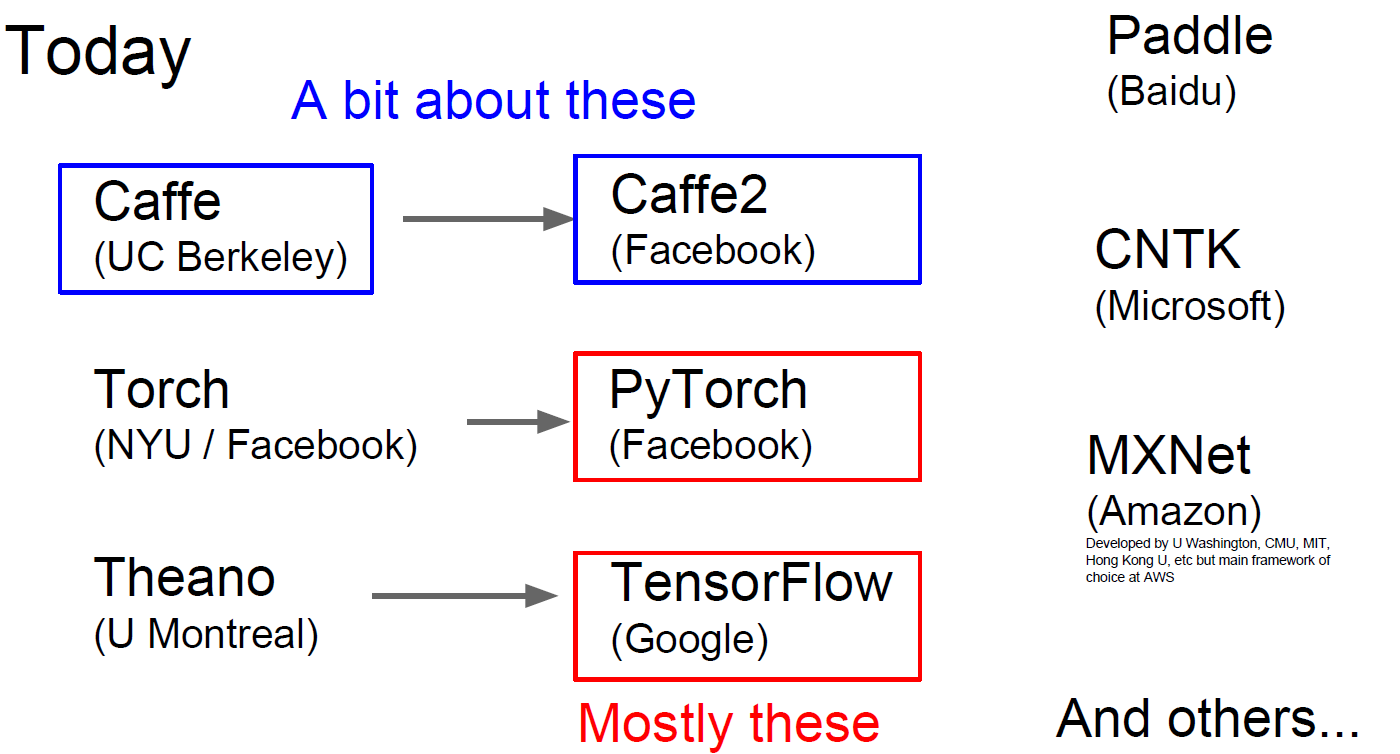
\includegraphics[width=0.8\textwidth]{fig/software}
\end{figure}

\section{Tasks}
\begin{enumerate}
	\item Given the data set in the first section, please implement a convolutional neural network to calculate the accuracy rate. The major steps involved are as follows:
	\begin{enumerate}
		\item Reading the input image.
		\item Preparing filters.
		\item Conv layer: Convolving each filter with the input image.
		\item ReLU layer: Applying ReLU activation function on the feature maps (output of conv layer).
		\item Max Pooling layer: Applying the pooling operation on the output of ReLU layer.
		\item Stacking conv, ReLU, and max pooling layers
	\end{enumerate}
	\item You can refer to the codes in \texttt{cs231n}. Don't use Keras, TensorFlow, PyTorch, Theano, Caffe, and other deep learning softwares.
	\item Please submit a file named \texttt{E16\_YourNumber.rar}, which should includes the code files and the result pictures, and send it to \texttt{ai\_201901@foxmail.com}
\end{enumerate}

\section{Codes and Results}
Following the steps described above, I glue different modules in \verb'cs231n' together.
\begin{enumerate}
	\item [(a)] To read the input images, I leverage the \verb'get_CIFAR10_data' function in \verb'data_utils.py', where it separate the data into training set, validation set, and test set, all of which are stored in a dictionary.
	Moreover, it normalizes the data for easy training later.
	The return data has the shape as follows,
\begin{flushleft}
X\_train:  (49000, 3, 32, 32)\\
y\_train:  (49000,)\\
X\_val:  (1000, 3, 32, 32)\\
y\_val:  (1000,)\\
X\_test:  (1000, 3, 32, 32)\\
y\_test:  (1000,)
\end{flushleft}
	Notice the channel dimension has been swap to axis 1 in numpy representation.

	\item [(b)] The filters are defined in \verb'layers.py'.
	The naive implementation of convolutional layer needs four nested loops.
	(Actually if counting the numpy summation implementation, there will be more loops.)
	In the innerest loop, the original image makes a dot product with the convolutional kernel.
\begin{lstlisting}
for ni in range(x.shape[0]):
    for fi in range(w.shape[0]):
        for xi in range(H_):
            for yi in range(W_):
                out[ni, fi, xi, yi] = np.sum(x_pad[ni, :, xi * stride:xi * stride + HH, yi * stride:yi * stride + WW] * w[fi, :, :, :])

        out[ni,fi,:,:]+=b[fi]
\end{lstlisting}

	The implementation of Max Pooling layer is similar, except for the max function.
	The key computation is listed below.
	The size of max pooling output is much easier to be calculated than the convolutional layer, since the stride is commonly set equal to the size of the max pooling kernel.
\begin{lstlisting}
for ni in range(x.shape[0]):
    for ci in range(x.shape[1]):
        for xi in range(H_):
            for yi in range(W_):
                out[ni, ci, xi, yi] = np.max(x[ni,ci,xi * stride:xi * stride + pool_height,yi * stride:yi * stride + pool_width])
\end{lstlisting}

	The backward pass of the convolutional layer and the max pooling layer are much harder than the forward pass, and the naive implementation also has great performance degradation.
	For example, backpropagation through max pooling layer needs to find the index that generates the current maximum, which needs a tedious traversal in each convolution.
	This is a large overhead if the traversal does not deal well.

	\item [(c,d,e,f)] Once the key components are built, what we need to do is to glue them.
	The CNN has been encapsulated as \verb'ThreeLayersConvNet' in \verb'cnn.py'.
	The architecture is defined below,
\begin{center}
conv - relu - 2x2 max pool - affine - relu - affine - softmax
\end{center}
	Then we directly call the forward pass and the backward pass of these layers, and the CNN will work properly.
	Notice the weights and biases should be stored when propagation in order to calculate the loss faster.
\end{enumerate}

After the three-layer CNN is built, I take the most of the \verb'Solver'.
Just instantiate the data and model, and pass them into the solver.
Press \verb'solver.train()', and the CNN will train automatically.
The codes are listed below.
\lstinputlisting{ConvNet.py}

I only train the CNN for three epochs, obtaining 55.8\% and 55\% of accuracy on train set and validation set representatively, as shown in Fig.~\ref{fig:acc}.
The accuracy on test set is 54.5\%.
\begin{figure}[H]
\centering
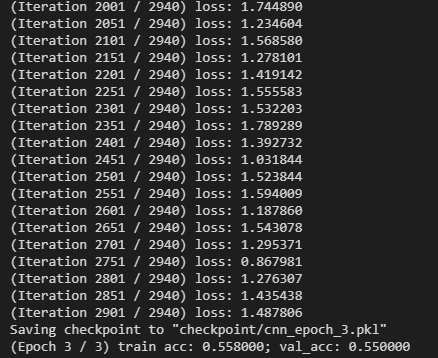
\includegraphics[width=0.6\linewidth]{fig/results/train_acc2.png}
\caption{Accuracy of train set and validation set}
\label{fig:acc}
\end{figure}

The training loss is shown in Fig.~\ref{fig:loss}.
\begin{figure}[H]
\centering
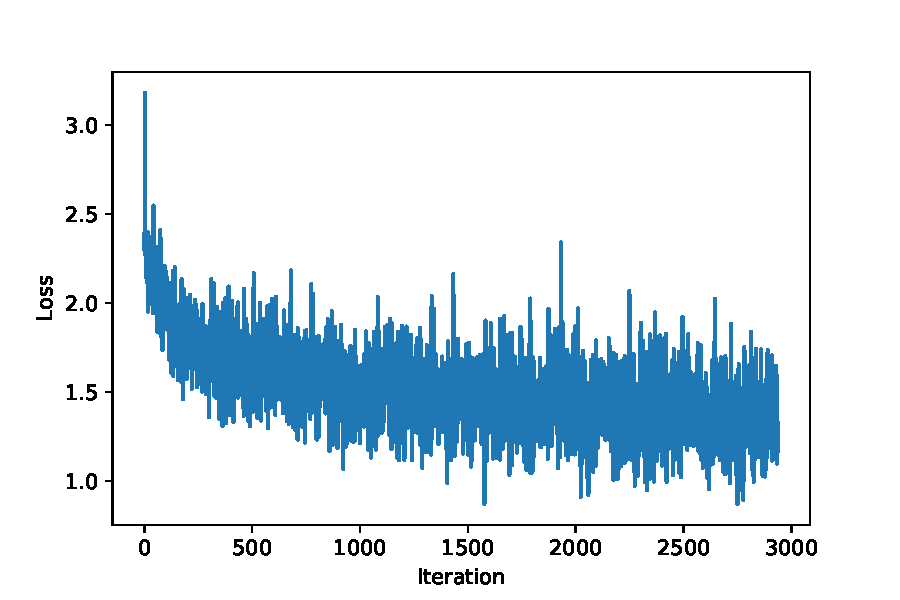
\includegraphics[width=0.5\linewidth]{fig/loss.pdf}
\caption{Training loss}
\label{fig:loss}
\end{figure}

From this experiment, I clearly realize that how slow the CPU is!
Even though the CIFAR dataset is such a toy dataset in nowadays deep learning research, it takes almost an hour to train only 3 epochs using my Intel i7 CPU, which is extremely unacceptable.
The code in \verb'cs231n' has been optimized using the ahead of time (AOT) compiler Cython.
However, the training process still takes a long time.
And we may know how much optimization has been done in Pytorch and Tensorflow, where C/C++ and Python codes are deeply fused.
Both of the frameworks greatly push the development of deep learning.
Moreover, the deployment of GPU in deep learning truly leads the AI field to take a big step.
That is why somebody said the Turing Award should be awarded to Jen-Hsun Huang, the CEO of Nvidia.

Moreover, we can observe a marginal effect decrement in Fig.~\ref{fig:loss}.
Actually after the first epoch, the CNN has reached 50\% accuracy on the train set.
The two more times of training only improve the performance for 5\%.
The investment and the return are not consistent.
This also makes us to think if it necessary to take so many resources to improve only little prediction accuracy in nowadays deep learning research, or this kind of improvement is just anything but useful.

At last, to summarize the AI course this term, I have to say this is the best course I have ever toke in SYSU.
Starting from simple searching algorithms, we got through logic, knowledge representation, planning, Bayes, and finally got the place of machine learning and deep learning.
Though the number of experiments is double of those of CS major, we learned a lot and built lots of artificial idiots, which is also a kind of fun!

Last but not least, great thanks to TAs, especially to Yukun :), who provide us lots of guidance on the road to the peak of artificial intelligence, and give us lots of happiness and warmness.

\end{document}